\documentclass[11pt]{article}

%  USE PACKAGES  ---------------------- 
\usepackage[margin=0.7in,vmargin=1in]{geometry}
\usepackage{amsmath,amsthm,amsfonts}
\usepackage{amssymb}
\usepackage{fancyhdr}
\usepackage{enumerate}
\usepackage{mathtools}
\usepackage{graphicx}
\usepackage{hyperref,color}
\usepackage{enumitem,amssymb}
\newlist{todolist}{itemize}{4}
\setlist[todolist]{label=$\square$}
\usepackage{pifont}
\newcommand{\cmark}{\ding{51}}%
\newcommand{\xmark}{\ding{55}}%
\newcommand{\done}{\rlap{$\square$}{\raisebox{2pt}{\large\hspace{1pt}\cmark}}%
\hspace{-2.5pt}}
\newcommand{\HREF}[2]{\href{#1}{#2}}
\usepackage{textcomp}
\usepackage{listings}
\lstset{
basicstyle=\small\ttfamily,
% columns=flexible,
upquote=true,
breaklines=true,
showstringspaces=false
}
%  -------------------------------------------- 

%  HEADER AND FOOTER (DO NOT EDIT) ----------------------
\newcommand{\problemnumber}{0}
\pagestyle{fancy}
\fancyhead{}
\fancyhead[L]{\textbf{Question \problemnumber}}
\newcommand{\newquestion}[1]{
\clearpage % page break and flush floats
\renewcommand{\problemnumber}{#1} % set problem number for header
\phantom{}  % Put something on the page so it shows
}
\fancyfoot[L]{IE 332}
\fancyfoot[C]{Assignment 2}
\fancyfoot[R]{Page \thepage}
\renewcommand{\footrulewidth}{0.4pt}

%  --------------------------------------------


%  COVER SHEET (FILL IN THE TABLE AS INSTRUCTED IN THE ASSIGNMENT) ----------------------
\newcommand{\addcoversheet}{
\clearpage
\thispagestyle{empty}
\vspace*{0.5in}

\begin{center}
\Huge{{\bf IE332 Assignment \#2}} % <-- replace with correct assignment #

Due: April 14th, 11:59pm EST % <-- replace with correct due date and time
\end{center}

\vspace{0.3in}

\noindent We have {\bf read and understood the assignment instructions}. We certify that the submitted work does not violate any academic misconduct rules, and that it is solely our own work. By listing our names below we acknowledge that any misconduct will result in appropriate consequences. 

\vspace{0.2in}

\noindent {\em ``As a Boilermaker pursuing academic excellence, I pledge to be honest and true in all that I do.
Accountable together -- we are Purdue.''}

\vspace{0.3in}

\begin{table}[h!]
  \begin{center}
    \label{tab:table1}
    \begin{tabular}{c|ccccc|c|c}
      Student & Q1 & Q2 & Q3 & Q4 & Q5 & Overall & DIFF\\
      \hline
      Talya Arpaci & 50 & 33 & 83 & 17 & 0 & 0 & 0\\
      Hershi Meher & 50 & 33 & 83 & 17 & 0 & 0 & 0\\
      Mohamed Abuelreish & 0 & 33 & 33 & -33 & 0 & 0 & 0\\
      Andrew Newquist & 50 & 33 & 83 & 17 & 0 & 0 & 0\\
      Nicholas Alfano & 0 & 33 & 33 & -33 & 0 & 0 & 0\\
      \hline
      St Dev & 29 & 0 & 29 & 29 & 0 & 0 & 0
    \end{tabular}
  \end{center}
\end{table}

\vspace{0.2in}

\noindent Date: \today.
}
%  -----------------------------------------

%  TODO LIST (COMPLETE THE FULL CHECKLIST - USE AS EXAMPLE THE FIRST CHECKED BOXES!) ----------------------
\newcommand{\addtodo}{
\clearpage
\thispagestyle{empty}

\section*{Read Carefully. Important!}

\noindent By electronically uploading this assignment to Brightspace you acknowledge these statements and accept any repercussions if in any violation of ANY Purdue Academic Misconduct policies. You must upload your homework on time for it to be graded. No late assignments will be accepted. {\bf Only the last uploaded version of your assignment before the due date will be graded}.

\vspace{0.2in}

\noindent {\bf NOTE:} You should aim to submit no later than 30 minutes before the deadline, as there could be last minute network traffic that would cause your assignment to be late, resulting in a grade of zero. 

\vspace{0.2in}

\noindent When submitting your assignment it is assumed that every student considers the below checklist, as there are grading consequences otherwise (e.g., not submitting a cover sheet is an automatic grade of ZERO).

\begin{todolist}

    \item[\done] Your solutions were prepared using the \LaTeX template provided in Brightspace. 
    \item[\done] Your submission has a cover sheet as its first page and this checklist as its second page, according to the template provided.
	 \item[\done] All of your solutions (program code, etc.) are included in the submission as requested. % Check this checkbox and the following ones if satisfied <---
    \item[\done] You have not included any screen shots, photos, etc. (plots should be intermediately saved as .png files and then added into your .tex file). % <---
	 \item[\done] All math notation and algorithms (algorithmic environment) are created using appropriate \LaTeX code (no pictures, handwritten solutions, etc.). % <---
    \item[\done] The .pdf is submitted as an individual file and not in a {\tt .zip}.
    \item[\done] You kept the \LaTeX source code in your files until this assignment is graded, in case you are required to show proof of creating your assignment using \LaTeX.  % <---
    \item[\done] If submitting with a partner, your partner is added in the submission section in Gradescope after you upload your file. % <---
    \item[\done] You have correctly matched each question to its page \# in the .pdf submission in the Gradescope section (after you uploaded your file).
    \item[\done] Watch videos on creating pseudocode if you need a refresher or quick reference to the idea. These are good starter videos:    % <---
    
     \HREF{https://www.youtube.com/watch?v=4jLO0vXPktU}{www.youtube.com/watch?v=4jLO0vXPktU} 
    
    \HREF{https://www.youtube.com/watch?v=yGvfltxHKUU}{www.youtube.com/watch?v=yGvfltxHKUU}
\end{todolist}
}

%% LaTeX
% Für alle, die die Schönheit von Wissenschaft anderen zeigen wollen
% For anyone who wants to show the beauty of science to others

%  -----------------------------------------


\begin{document}


\addcoversheet

\addtodo

% BEGIN YOUR ASSIGNMENT HERE:
\newpage

\fancyhead[L]{\textbf{Question 1}}
\section{Question 1}
% Question 1

% \noindent Example of proper typesetting of quotation marks:\\
% ``proper opening and closing quotation marks'' vs "bad quotation marks".
\subsection{Part A}
ENTER HERE

\subsection{Part B}
Part B Written Explanation:
Because of their constant time complexity, lines 1 and 6 can be disregarded for analysis.
For each iteration of the outer loop (line 2), which itself iterates n times, the inner loop (lines 3 to 5) iterates sqrt(n) times. As a result, the inner loop is run n*sqrt(n) times in total.
Each iteration of the inner loop requires a constant amount of time because h(j)'s complexity is $\theta$ (1). As a result, the algorithm's overall time complexity is (n*sqrt(n)).
We can omit the lower-order term sqrt(n) in large O notation, making the time complexity O(n*sqrt(n)). Similarly, we can write the time complexity as (n*sqrt(n)) in the Theta notation.
In conclusion, the algorithm presented has a time complexity of (n*sqrt(n)).

\subsection{Part C}
ENTER HERE

\subsection{Part D}
Part D Written Explanation:
The time complexity of this algorithm depends on the value of the input number x. Let's analyze the three cases:
1 - If x is a power of 2:
The algorithm will run in log(x) time if x is a power of two since it will iterate over the while loop log(x) times, dividing each time by 2 until the result is 1. Since x is not divisible by 3, the function g(X) is not invoked in this situation.

2 - If x is divisible by 3 but not divisible by 2:
Similar to the prior example, the algorithm will execute in log(x) time, but this time, each iteration will now include a check to verify if x is divisible by 3. If so, x is set to be 2 to the power of x and the function g(X) is not called. Instead, dividing x by 2 is performed by calling the function g(X). The algorithm's overall time complexity in this situation is still O(log(x)), as the function g(X) runs in log(x) time.

3 - If x is not a power of 2 and not divisible by 3:
As there is no condition to stop the loop in this instance, the algorithm will continue to loop forever. Given that x must be an integer with a value larger than 1, we may assume that this scenario won't occur.

Therefore, the time complexity of the algorithm is O(log(x)).
As for the space complexity, it is constant since the algorithm does not use any extra memory that grows with the input size.


\subsection{Part E}

ENTER HERE


\subsection{Part F}

ENTER HERE


\subsection{Part G}

ENTER HERE
\newpage

% Question 2
\fancyhead[L]{\textbf{Question 2}}
\section{Question 2}
\subsection{Part A}

Part A Written Explanation:
The loop invariant is i<x which makes the code run (as long as i is less than the amount of attempts run the code). This  condition holds true throughout the code. The loop in variants seem to be correct. 


\subsection{Part B}
Part B R Code:
\begin{lstlisting}[language=R, frame=single]
library(purrr)

f <- function(x) {
  count <- 0
  i <- 0
  while (i < x) {
    xcyc <- map_dbl(rep(runif(1,-1,1), 2), `^`, 2)
    if (sum(xcyc) < 1) {
      count <- count + 1
    }
    i <- i + 1
  }
  print(count/i*4)
}
\end{lstlisting}

\subsection{Part C}
Part C R Code:
\begin{lstlisting}[language=R, frame=single]
library(purrr)
f <- function(x, count=0, i=0){
  xcyc =map_dbl(rep(runif(1,-1,1), 2), `^`, 2)
  if (sum(xcyc)<1) {
  count<-count+1
  }
  i<-i+1
  if (i<x)
  return(f(x, count, i))
  else{
    return(count/i*4)
  }
}
\end{lstlisting}
Part C Written Explanation:

In the original case i<x is a while loop condition that runs until the code has run out of attempts
In this case i<x is an if statement, serving as a guard expression. Recursivity is put into an if statement with a loop condition i<x that returns to the initial function by passing x, count and i variables to its next iteration within the function. With every recursive run i larger and once it  gets equal to x,it puts a stop to the function and returns the final result of the code. 

Let us try to prove the correctness of this code.
Initialization: Once we enter the code with x attempts, count =0 and i=0  the code will generate a random point within -1,1 and square them. At this stage is i<x. Then if the sum of the coordinates is less then 1 the count increases by 1 with an afterwards increase of i
Maintenance: To see that each iteration maintains i<x, observe how i changes  and compare it to x. Once the condition i<x holds true then we return to the function with the same value of x and the new increased count and i. The next iteration is entered with x, count=1 and i=1. Termination: Eventually, having this process repeated i will become equal to x and the condition (i<x) terminates, leading to the else statement return(count/i*4) . Which means that invariant i<x still holds true.
\newpage

% Question 3
\fancyhead[L]{\textbf{Question 3}}
\section{Question 3}
\subsection{Part A}
ENTER HERE
\subsection{Part B}
ENTER HERE
\subsection{Part C}
ENTER HERE
\subsection{Part D}
ENTER HERE
\subsection{Part E}
ENTER HERE
\subsection{Part F}
ENTER HERE
\subsection{Part G}
ENTER HERE
\newpage

% Question 4
\fancyhead[L]{\textbf{Question 4}}
\section{Question 4}
\subsection{Part A}
Part A Written Explanation: 
Over 10 epochs for the less complex neural network comprised of 5 nodes and 1 hidden layer, there seems to be a net under-fitting when comparing the performances of the test and training results in Figure 1. This result was to be expected as under-fitting occurs when a model is too simple. This model proved to be too simple.
Part A R Code:
\begin{lstlisting}[language=R, frame=single]
library(neuralnet)
#Import the data and clean it of Na's. Convert neg,pos to 0,1.
aps_failure_data <-
  read.csv("aps_failure_training_set.csv", na.strings = c("", "na"))
aps_failure_data_clean <- na.omit(aps_failure_data)
aps_failure_data_clean$class <-
  ifelse(aps_failure_data_clean$class == "pos", 1, 0)
#Define training and testing data
training_data <- aps_failure_data_clean[1:295,]
testing_data <- aps_failure_data_clean[296:590,]
# Creates the neural net with the training data hidden = changes the complexity
#to compare performance over epochs
neural_net4a <-
  neuralnet(class ~ . - training_data$class,data = training_data,hidden = c(25,5),
    linear.output = FALSE,algorithm = "sag")
#Initialize variables to track errors
training_errors <- rep(0, 10)
testing_errors <- rep(0, 10)
#Loop over the number of epochs to collect errors
for (i in 1:10) {
#Compute errors on training data
  net_result_train <- compute(neural_net4a, training_data[])
  training_errors[i] <-sum((net_result_train$net.result[, 1] > 0.5)!= training_data[, "class"])
#Compute errors on testing data
  net_result_test <- compute(neural_net4a, testing_data[])
  testing_errors[i] <- sum((net_result_test$net.result[, 1] > 0.5)!= testing_data[, "class"])
#Update the neural network with training data
  neural_net4a <- update(neural_net4a, training_data[],training_data[, "class"])
}
#Plots the training and testing errors over the epochs
plot(training_errors,type = "l",col = "blue",xlab = "# of Epochs",ylab = "# of Errors",
  ylim = c(0, max(training_errors, testing_errors)),main = "Panel 2")
lines(testing_errors, type = "l", col = "red")
legend("bottomright",legend = c("Training Errors", "Testing Errors"),col = c("blue", "red"),lty = 1)
\end{lstlisting}

\subsection{Part B} 
Part B Written Explanation: 
As the complexity of the neural net increased, the under-fitting behavior approached a more over-fitting behavior. In Figure 3, the fit appeared to be closest to its 'sweet spot', which is typically seen in the classical U-shaped risk curve. However, after that point, as the complexity increased in Figure 4, an over-fitting behavior began to appear, putting the test at risk. The complexity at this point was too high to accurately predict new data. The algorithm reached the point of memorization rather than learning. 

\begin{figure}[!tbp]
  \centering
  \begin{minipage}[b]{0.4\textwidth}
    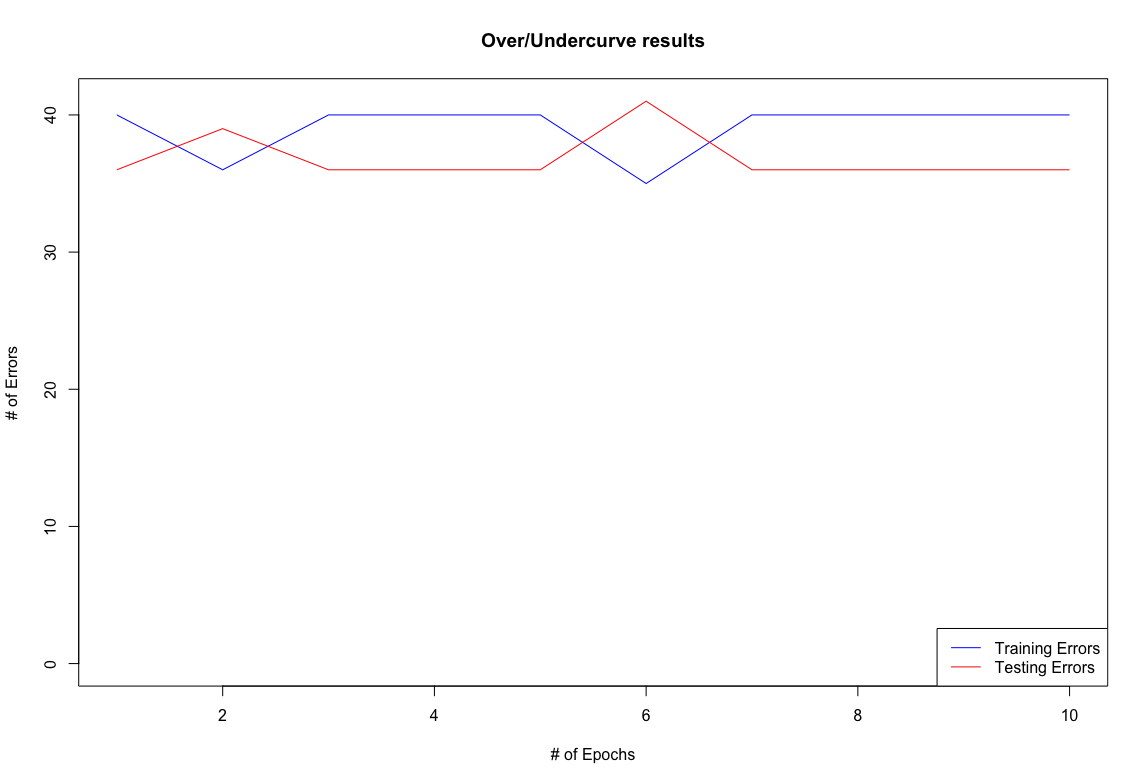
\includegraphics[width=\textwidth]{Complexity 1.png}
    \caption{Hidden Nodes:5   Hidden Layers:1}
  \end{minipage}
  \hfill
  \begin{minipage}[b]{0.4\textwidth}
    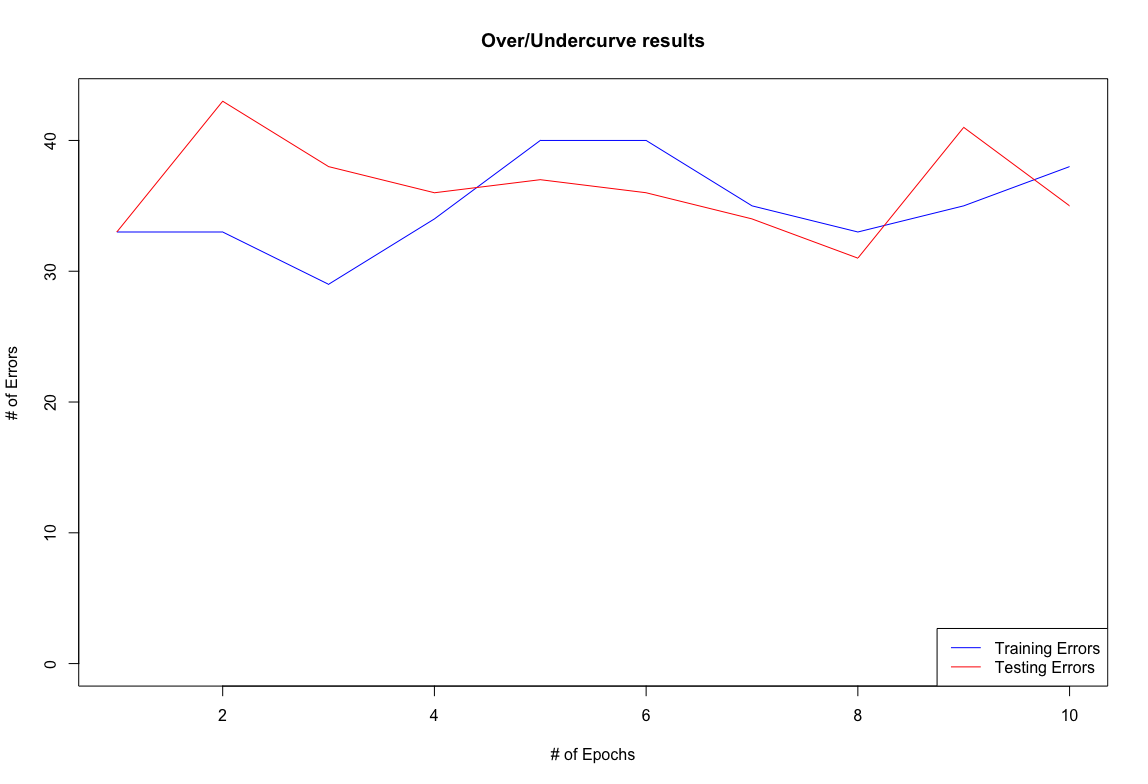
\includegraphics[width=\textwidth]{Complexity2.png}
    \caption{Hidden Nodes:10   Hidden Layers:1}
  \end{minipage}
\end{figure}
\begin{figure}[!tbp]
  \centering
  \begin{minipage}[b]{0.4\textwidth}
    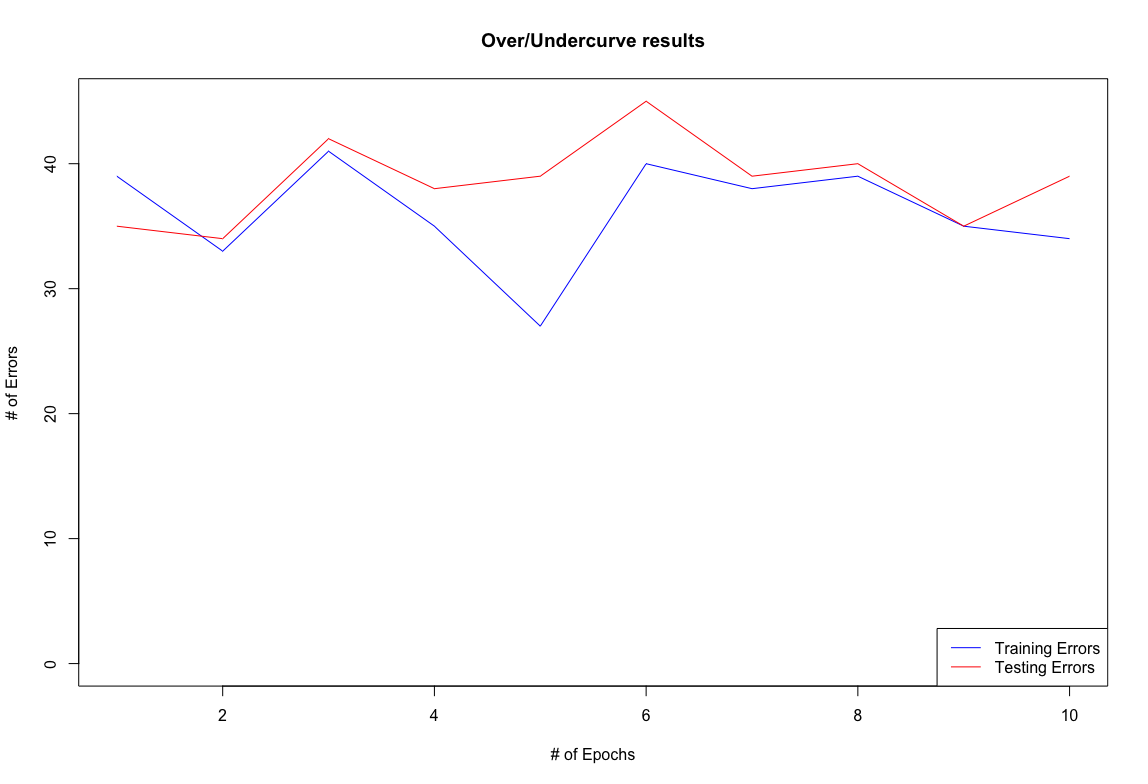
\includegraphics[width=\textwidth]{Complexity3.png}
    \caption{Hidden Nodes:10   Hidden Layers:2}
  \end{minipage}
  \hfill
  \begin{minipage}[b]{0.4\textwidth}
    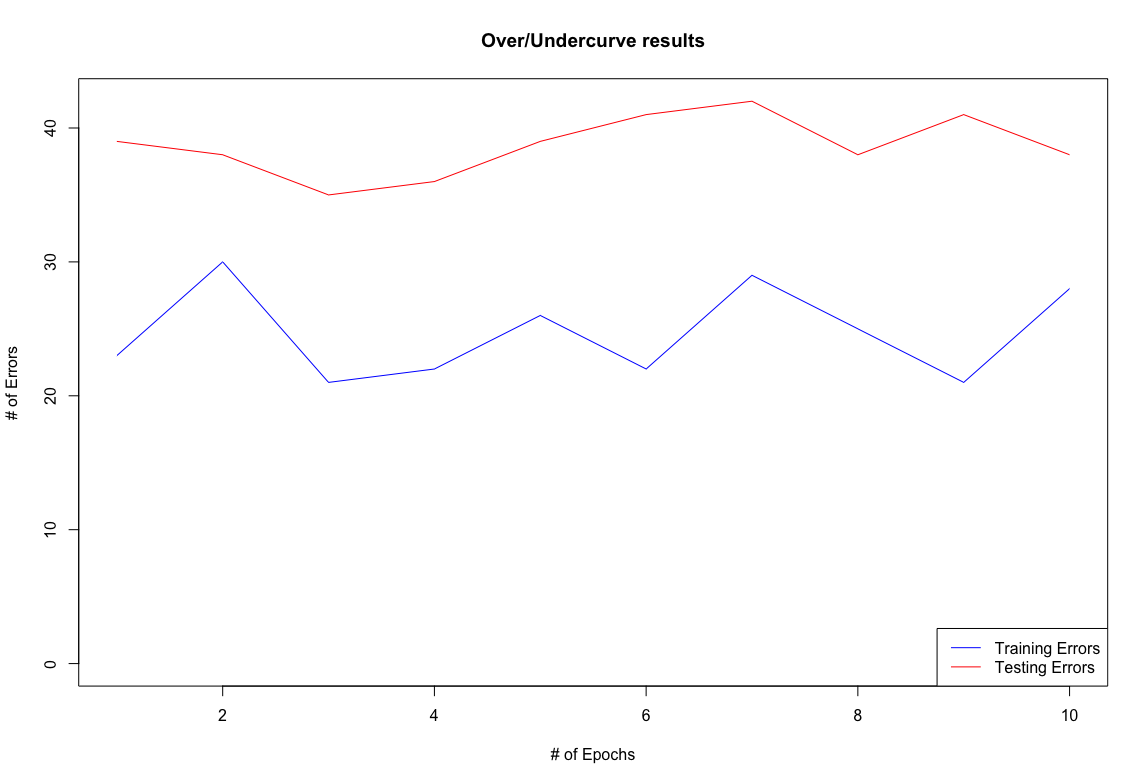
\includegraphics[width=\textwidth]{Complexity4.png}
    \caption{Hidden Nodes:25   Hidden Layers:2}
  \end{minipage}
\end{figure}


\subsection{Part C} 
ENTER HERE

\newpage
% Question 5
\fancyhead[L]{\textbf{Question 5}}
\section{Question 5}
Libraries used for Question 5:
\begin{lstlisting}[language=R, frame=single]
library(tidyverse)
library(cluster)
library(factoextra)
library(gridExtra)
library(dplyr)
library(caret)
library(car)
library(glmnet)
\end{lstlisting}
\subsection{Part A} 
Part A R Code:
\begin{lstlisting}[language=R, frame=single]
#Import Data. Ensure this .r file is in the same folder/working directory as the .csv
real_estate_data_raw <- read.csv("train.csv", header=TRUE)


#Clean data. Remove NAs, scale, and select only numerical columns. Remove Zero variance columns
real_estate_data <-select_if(real_estate_data_raw, is.numeric)
re_data_frame<- na.omit(real_estate_data)
re_data_frame<- re_data_frame[sample(nrow(re_data_frame),50),] #  <----- THIS IS AMOUNT OF PROPERTIES TO BE INCLUDED IN CLUSTERING
Var <- apply(re_data_frame, 2, var)
zero_var_col <- which (Var == 0)
re_data_frame<- re_data_frame[, -zero_var_col]

#Create Cluster.
cluster3 <- kmeans(re_data_frame, centers = 4, nstart = 5)
#Collect Individual Cluster Data
cluster1_data <- re_data_frame[cluster3$cluster == 1, ]
cluster2_data <- re_data_frame[cluster3$cluster == 2, ]
cluster3_data <- re_data_frame[cluster3$cluster == 3, ]
cluster4_data <- re_data_frame[cluster3$cluster == 4, ]
c1qual <- mean(cluster1_data$OverallQual)
c2qual <- mean(cluster2_data$OverallQual)
c3qual <- mean(cluster3_data$OverallQual)
c4qual <- mean(cluster4_data$OverallQual)

#Plots the Clusters. Prints Average Quality of cluster
plot3 <-fviz_cluster(cluster3, data = re_data_frame)
grid.arrange(plot3)
cat("The Average Overall Quality Rating of Cluster 1 is", sprintf("%.2f", c1qual))
cat("The Average Overall Quality Rating of Cluster 2 is", sprintf("%.2f", c2qual))
cat("The Average Overall Quality Rating of Cluster 3 is", sprintf("%.2f", c3qual))
cat("The Average Overall Quality Rating of Cluster 4 is", sprintf("%.2f", c4qual))

\end{lstlisting}
\subsection{Part B} 
Part B Written Explanation:
After the clustering algorithm executes, the data of all 4 clusters is collected. The script then analyzes this data to provide a printing of the average overall quality of each cluster’s properties. This is a strong predictor of an increase in real-estate prices. A prospective buyer is looking for an investment, and a piece of real estate with excellent overall quality would be the target of the said buyer. The clusters are created from a random selection of 50 properties from the overall data set so that the cluster remains readable but contains enough data to be useful. Whichever cluster has the highest overall quality is likely to increase in price. 
\subsection{Part C} 
Part C Written Explanation:
The regression machine learning algorithm used for all numerical real-estate data saw an r-squared value of 0.765. This value shows a high correlation between the predicted values and the actual values in the testing data set used for the algorithm. The group regards this as a positive result regarding the performance of our linear regression model. The model we used predicted the overall quality of the properties.
Part C R Code:
\begin{lstlisting}[language=R, frame=single]
#Regression machine learning algorithm on all data for overall quality of
#property 5C--------------------------------------------------------------------
#Creating Training Data
training <- real_estate_data[1:730,]
training <- na.omit(training)
training <- training[1:550,]

#Creating Testing Data
testing <- real_estate_data[731:1460,]
testing <- na.omit(testing)
testing <- testing[1:550,]

#Fitting Model to predict overall quality
reg_model <- lm(training$OverallQual~.-training$Id -training$MSSubClass,data = training)

#Testing Model ability to predict overall quality
predictions <- predict(reg_model, newdata = testing)
Rsquare <- sqrt(mean((testing$OverallQual - predictions)^2))
print(paste0("R-squared value is: ", round(Rsquare, 3)))
\end{lstlisting}

\subsection{Part D} 
Part D Written Explanation:
The regression machine learning algorithm used for the individual clusters of real-estate data was an altered version of the algorithm used in part 5c. Instead of using all the data, the algorithm collected the data from each cluster in a data frame as the clusters are constructed. The group wanted to test and train with an equal amount of rows of data, so if a cluster had an odd amount of data entities, then one was omitted to allow for an even, whole-numbered split. The clusters saw anywhere between 0.69 - 0.78 r-squared values when the algorithm is run and clusters were created. These results are seen as positive. However, the group made notice of an anomaly that occurred when the script is executed. One of the clusters had an r-squared value of 32. As R-squared values should be between 0-1, this is an inaccurate prediction for that specific cluster. Despite debugging efforts, the group could not reach the issue's root.

Part D R Code:
\begin{lstlisting}[language=R, frame=single]
#Regression machine learning algorithm on individual cluster data for overall 
#quality of property 5D------------------------------------------------------------

#Collect Individual Cluster Data
cluster1_data <- re_data_frame[cluster_alg$cluster == 1, ]
cluster2_data <- re_data_frame[cluster_alg$cluster == 2, ]
cluster3_data <- re_data_frame[cluster_alg$cluster == 3, ]
cluster4_data <- re_data_frame[cluster_alg$cluster == 4, ]

#Determine size of Test and Train data frames for each cluster. If even, split. If odd ommit 1 and split
cluster11_counts <- nrow(cluster1_data)
if (cluster11_counts %% 2 == 1) {
  cluster12_counts <- floor((cluster11_counts - 1) / 2)
} else {
  cluster12_counts <- cluster11_counts / 2
}

cluster21_counts <- nrow(cluster2_data)
if (cluster21_counts %% 2 == 1) {
  cluster22_counts <- floor((cluster21_counts - 1) / 2)
} else {
  cluster22_counts <- cluster21_counts / 2
}

cluster31_counts <- nrow(cluster3_data)
if (cluster31_counts %% 2 == 1) {
  cluster32_counts <- floor((cluster31_counts - 1) / 2)
} else {
  cluster32_counts <- cluster31_counts / 2
}

cluster41_counts <- nrow(cluster4_data)
if (cluster41_counts %% 2 == 1) {
  cluster42_counts <- floor((cluster41_counts - 1) / 2)
} else {
  cluster42_counts <- cluster41_counts / 2
}

#Creating Training and Testing Data Data Cluster 1,2,3,4
training_c1 <- cluster1_data[1:cluster12_counts,]
testing_c1 <- cluster1_data[(cluster12_counts+1):cluster11_counts,]
training_c2 <- cluster2_data[1:cluster22_counts,]
testing_c2 <- cluster2_data[(cluster22_counts+1):cluster21_counts,]
training_c3 <- cluster3_data[1:cluster32_counts,]
testing_c3 <- cluster3_data[(cluster32_counts+1):cluster31_counts,]
training_c4 <- cluster4_data[1:cluster42_counts,]
testing_c4 <- cluster4_data[(cluster42_counts+1):cluster41_counts,]

#Fitting each cluster a regression model to predict overall quality
reg_model_c1 <- lm(training_c1$OverallQual~.,data = training_c1)
reg_model_c2 <- lm(training_c2$OverallQual~.,data = training_c2)
reg_model_c3 <- lm(training_c3$OverallQual~.,data = training_c3)
reg_model_c4 <- lm(training_c4$OverallQual~.,data = training_c4)

#Test the Models ability to predict overall quality
predictions_c1 <- predict(reg_model_c1, newdata = testing_c1)
Rsquare_c1 <- sqrt(mean((testing_c1$OverallQual - predictions_c1)^2))
print(paste0("R-squared value for the cluster 1 model is: ", round(Rsquare_c1, 3)))
predictions_c2 <- predict(reg_model_c2, newdata = testing_c2)
Rsquare_c2 <- sqrt(mean((testing_c2$OverallQual - predictions_c2)^2))
print(paste0("R-squared value for the cluster 2 model is: ", round(Rsquare_c2, 3)))
predictions_c3 <- predict(reg_model_c3, newdata = testing_c3)
Rsquare_c3 <- sqrt(mean((testing_c3$OverallQual - predictions_c3)^2))
print(paste0("R-squared value for the cluster 3 model is: ", round(Rsquare_c3, 3)))
predictions_c4 <- predict(reg_model_c4, newdata = testing_c4)
Rsquare_c4 <- sqrt(mean((testing_c4$OverallQual - predictions_c4)^2))
print(paste0("R-squared value for the cluster 4 model is: ", round(Rsquare_c4, 3)))
\end{lstlisting}
\end{document}
